%###
% \RequirePackage[l2tabu, orthodox]{nag}
\documentclass[a4paper,10pt,twoside]{book}
% \usepackage[width=127mm,height=191mm,includehead,hcentering,vcentering]{geometry}

% \includeonly{_init,basic-concepts,raster}
% \includeonly{__init,k3tree}

% Packages --------------------------------------------------------------------

\usepackage{booktabs,multirow,multicol,array,colortbl,makecell,tabularx} % tablas


\usepackage[width=127mm,height=191mm,includehead,hcentering,vcentering]{geometry}
\usepackage{graphicx,subfigure}				% Include graphics
\usepackage{caption}	% Customize captions
\usepackage[T1]{fontenc} 			% Extended character set
\usepackage{lmodern, microtype}		% Load vector fonts; better text formatting
\usepackage{amsmath,amssymb,amsfonts,amsthm}	% Math support, example environment
\usepackage{fancyhdr} 				% Headers
\usepackage{xspace}	  				% Create macros with appropriate extra space after
\usepackage{lipsum}					% Fill sections
\usepackage{fixltx2e}				% Make math macros robust: \( \) \[ \]



\usepackage[usenames,dvipsnames]{xcolor}	% Colors

\usepackage[chapter]{algorithm}
\usepackage{algorithmicx, algpseudocode}
\usepackage{float}

\usepackage{textcomp, gensymb}	% Common symbols (mu, degree)

%Debug packages
% \usepackage{refcheck}	% Show labels in output pdf. 
						% Note: local refcheck.sty has been modified to solve a bug in handling bibitems 
						% Note 2: since cleveref refcheck is unused




\usepackage{tikz}

\usepackage[breaklinks]{hyperref} % Hyperlinks in refs. Must be loaded at the end (except cleverref)
\usepackage{hypdvips}
% \usepackage[nameinlink]{cleveref}
\usepackage{cleveref}

% \usepackage{theorem}					% Theorems?
% \theoremstyle{plain}
% \newtheorem{definition}{Definition}

% \usepackage{lscape} 					% Set elements to landscape (e.g large figures, tables)
% \usepackage{setspace}					% ??
% \usepackage{rotating}
% \usepackage[tight]{subfigure}
% \usepackage{dcolumn}
% \usepackage[noline,linesnumbered,algochapter]{algorithm2e}
% \providecommand{\DontPrintSemicolon}{\dontprintsemicolon}
% \usepackage{algcompatible}
% \usepackage{sectsty}
%\usepackage[none]{hyphenat}
% \usepackage[tworuled,noline,linesnumbered,algochapter]{algorithm2e}


% FIXME: review in further versions
\hyphenpenalty=5000
\tolerance=1000
\widowpenalty=300
\clubpenalty=300
\emergencystretch=3em

\hfuzz=3em

\usepackage{etoolbox}
\apptocmd{\sloppy}{\hbadness 10000\relax}{}{}	% Avoid ''underfull hbox'' warnings in bibliography


% Separacion entre un parrafo y el siguiente
% \addtolength{\smallskipamount}{-7.60pt}
% \addtolength{\parskip}{.5\baselineskip}%{.5\baselineskip}

% \setlength{\smallskipamount}{-7.60pt}
% \setlength{\parskip}{\smallskipamount}

% Fuente de las subsubsecciones
%\subsubsectionfont{\bf}

\setcounter{tocdepth}{4} \setcounter{secnumdepth}{4}

% Fuentes de los pies de figura
\renewcommand{\captionlabelfont}{\bfseries}
\setlength{\captionmargin}{\parindent}

\renewcommand{\arraystretch}{1.2}	% Adjust vertical margins in tables

%Comandos

\newcounter{example}[chapter]
\def\theexample{\thechapter.\arabic{example}}
\newenvironment{example}{\par\noindent\textbf{Example \refstepcounter{example}\theexample:}}{}

% I need subsubsubsections, but not in the index
\newcommand{\subsubsubsection}[1]{\vspace{2mm}\par\noindent\textbf{#1}}

\renewcommand{\algorithmicrequire}{\textbf{Input:}}
\renewcommand{\algorithmicensure}{\textbf{Output:}}
\newcommand{\Input}{\Require}
\newcommand{\Output}{\Ensure}
\newcommand{\false}{\textbf{false}}
\newcommand{\red}[1]{{\color{red} #1 }}
\newcommand{\blue}[1]{{\color{blue} #1 }}
\newcommand{\cyan}[1]{{\color{cyan} #1 }}
\newcommand{\green}[1]{{\color{green} #1 }}
\newcommand{\todo}[1]{\blue{#1}}
\newcommand{\rewrite}[1]{\cyan{#1}}
\newcommand{\fixme}[1]{{\Large \red{#1}}}

\newcommand*{\irank}[0]{\emph{rank}\xspace}
\newcommand*{\iselect}[0]{\emph{select}\xspace}
\newcommand*{\iaccess}[0]{\emph{access}\xspace}

\DeclareMathOperator\rank{rank}
\DeclareMathOperator\select{select}
\DeclareMathOperator\access{access}

\renewcommand*{\k}[0]{\ensuremath{K}\xspace}
\newcommand*{\kk}[0]{\ensuremath{\k^2}\xspace}
\newcommand*{\kkk}[0]{\ensuremath{\k^3}\xspace}
\newcommand*{\KK}[0]{\ensuremath{\K^2}\xspace}
\newcommand*{\Ktree}[0]{\ensuremath{\k^2}-tree\xspace}
\newcommand*{\ktree}[0]{\ensuremath{\k^2}-tree\xspace}
\newcommand*{\ktrees}[0]{\ensuremath{\k^2}-trees\xspace}
\newcommand*{\Ktrees}[0]{\ensuremath{\k^2}-trees\xspace}
\newcommand*{\koct}[0]{\ensuremath{\k^3}-tree\xspace}
\newcommand*{\Koct}[0]{\ensuremath{\k^3}-tree\xspace}
\newcommand*{\kntree}[0]{\ensuremath{\k^n}-tree\xspace}
\newcommand*{\Kntree}[0]{\ensuremath{\k^n}-tree\xspace}
\newcommand{\kones}[0]{\ensuremath{\k^2}-tree1\xspace}
\newcommand{\koness}[0]{\ensuremath{\k^2}-tree1s\xspace}
\newcommand{\Kones}[0]{\kones}
\newcommand{\kdouble}[0]{\ensuremath{\k^2}-tree1\ensuremath{^{\mathrm{2bits-naive}}}\xspace}
\newcommand{\ksus}[0]{\ensuremath{\k^2}-tree1\ensuremath{^{\mathrm{2bits}}}\xspace}
\newcommand{\kdf}[0]{\ensuremath{\k^2}-tree1\ensuremath{^{\mathrm{df}}}\xspace}
\newcommand{\klevel}[0]{\ensuremath{\k^2}-tree1\ensuremath{^{\mathrm{1-5 bits}}}\xspace}
\newcommand{\Kdouble}[0]{\kdouble}
\newcommand{\Ksus}[0]{\ksus}
\newcommand{\Kdf}[0]{\kdf}
\newcommand{\Klevel}[0]{\klevel}
\newcommand{\btree}[0]{B-tree\xspace}
\newcommand{\btrees}[0]{B-trees\xspace}
\newcommand{\bplus}[0]{B\ensuremath{^+}-tree\xspace}
\newcommand{\bpluss}[0]{B\ensuremath{^+}-trees\xspace}
\newcommand{\dktree}[0]{d\ktree}
\newcommand{\dktrees}[0]{d\ktrees}
\newcommand{\Dktree}[0]{D\ktree}
\newcommand{\Dktrees}[0]{D\dtrees}
\newcommand{\iktree}{I\ktree}
\newcommand{\diktree}{diff-I\ktree}
\newcommand{\mktree}{M\ktree}

\newcommand{\kkind}{M\kones}
\newcommand{\kkacum}{AM\kones}
\newcommand{\ikones}{I\kones}
\newcommand{\koctindex}{\koct}

\newcommand{\diffk}[0]{diffK}
\newcommand{\ediffk}[0]{enh-diffK}
\newcommand{\Diffk}[0]{DiffK}
\newcommand{\Ediffk}[0]{Enh-diffK}

\newcommand{\ktreap}[0]{\ensuremath{\k^2}-treap\xspace}
\newcommand{\ktreaps}[0]{\ensuremath{\k^2}-treaps\xspace}

\newcommand{\ZERO}[0]{0\xspace}
\newcommand{\ZEROS}[0]{0's\xspace}
\newcommand{\ONE}[0]{1\xspace}
\newcommand{\ONES}[0]{1s\xspace}

\newcommand{\dash}[0]{\text{--}}

\newcommand{\kt}[0]{\ensuremath{k}\xspace}

\newcommand{\tdktree}[0]{tt\ktree}


\crefname{algorithm}{Algorithm}{Algorithms}
\crefname{example}{Example}{Examples}
\crefname{part}{Part}{Parts}
\crefname{table}{Table}{Tables}

% \normalfont
% \DeclareFontShape{T1}{lmr}{bx}{sc} { <-> ssub * cmr/bx/sc }{}

\normalfont
\DeclareFontShape{T1}{lmr}{bx}{sc} { <-> ssub * cmr/bx/sc }{}

%%%%%%%%%%%%%%%%%%%%%%%%%%%%%%%%%%%%%%%%%%%%%%%%%%%%%%%%%%%
%%%%%%%%%%%%%%%% Sandbox
% \DeclareSymbolFont{sfoperators}{OT1}{cmss}{m}{n}
% \DeclareSymbolFontAlphabet{\mathsf}{sfoperators}
% 
% \makeatletter
% % \def\operator@font{\mathgroup\symsfoperators}
% \def\select@font{\mathgroup\symsfoperators}
% \makeatother
% 
% \makeatletter
% \def\rank@font{\sf}
% \def\select@font{\bf}
% \makeatother

% \newcommand{\rank}[0]{\ensuremath{\mathrm{rank}}\xspace}
% \newcommand{\select}[0]{\ensuremath{\mathrm{select}}\xspace}
% \newcommand{\irank}[0]{\emph{rank}\xspace}
% \newcommand{\iselect}[0]{\emph{select}\xspace}
% \def\rank{\ensuremath{\mathsf{rank}}}
% \def\select{\ensuremath{\mathsf{select}}}
% \DeclareMathOperator\rank{rank}
% \DeclareMathOperator\select{select}

%%%%%%%%%%%%%% End sandbox
%%%%%%%%%%%%%%%%%%%%%%%%%%%%%%%%%%%%%%%%%%%%%%%%%%%%%

\makeglossaries

\begin{document}

\pagenumbering{roman}
\pagestyle{fancy}\fancyfoot{}\fancyhead{}
\fancyhead[LO]{\slshape\nouppercase{\rightmark}}
\fancyhead[RE]{\slshape\nouppercase{\leftmark}}
\fancyhead[RO,LE]{\slshape \thepage}

\frontmatter

\newacronym{afc}{AFC}{Automated Fare Collection}
\newacronym{gis}{GIS}{Geographic Information System}
\newacronym{csa}{CSA}{Compressed Suffix Array}
\newacronym{wt}{WT}{Wavelet Tree}
\newacronym{wm}{WM}{Wavelet Matrix}
\newacronym{htwt}{HTWT}{Hu-Tucker Wavelet Tree}
\newacronym{ctr}{CTR}{Compact Trip Representation}
\newacronym{gtfs}{GTFS}{General Transit Feed Specification}
\newacronym{sat}{SAT}{Summed Area Table}
\newacronym{ttctr}{TTCTR}{Topology\&Trip-aware Compact Trip Representation}
\newacronym{xctr}{XCTR}{eXtended Compact Trip Representation}
\newacronym{tm}{T-Matrices}{Trip-Matrices}
\newacronym{dbms}{DBMS}{Database Management System}
\newacronym{rdbms}{RDBMS}{Relational Database Management System}
\newacronym{wms}{WMS}{Web Map Service}
\newacronym{wfs}{WFS}{Web Feature Service}
\begin{titlepage}


\vspace*{0.9cm}

\noindent {\Huge Compressed Data Structures\\ for Trajectory Representation}

\vspace*{1.5cm}

\noindent {\huge Autor: Daniil Galaktionov Hodovaniuk}


\definecolor{rosaudc}{RGB}{198, 0, 126}
\noindent \textcolor{rosaudc}{\rule{\textwidth}{2mm}}

{\large
  \noindent Tesis doctoral UDC / 2019

  \vspace*{1.5cm}

  \noindent Directores: \\Antonio Fari\~na Mart\'inez \\ Nieves Rodr\'iguez Brisaboa
  
  \vspace*{1.0cm}
  
  \noindent Tutor y Director por parte de la empresa: \\Eduardo Rodr\'iguez L\'opez

  \vspace*{1.5cm}

 % \noindent Programa Oficial de Doutoramento en Computaci\'on
}

\begin{center}
  \vspace*{1.9cm}
  
\includegraphics[scale=0.20]{figures/_init/udc-color}
\end{center}


\end{titlepage}

\thispagestyle{empty}

%\begin{titlepage}
%\begin{center}
%
%%\vspace*{0.9cm}
%
%
\includegraphics[scale=0.30]{figures/_init/udc-color}
%
%\vspace*{1.2cm}
%
%%{\large \sc Departamento de Computaci\'on, Universidade da Coru\~na} \\[5mm]
%%{\large \scshape Departamento de Computaci\'on} \\[5mm]
%%{\large } \\[2mm]
%%{\Large \scshape Proyecto fin de carrera \\ de Ingenier�a Inform�tica} \\
%
%\vspace*{2.5cm}
%
%{\LARGE \textsc{\textbf Compact data structures for large and complex datasets}}
%
%\end{center}
%
%\vspace*{2.8cm}
%
%\begin{center}
%%\large \bf
%\large
%{\Large \textsc{\textbf{Tesis Doctoral}}} \\[1.8cm]
%{{Doctorando:}  %\\[2mm]
%Fernando Silva Coira}\\[4mm]
%{{Directores:} %\\[2mm]
%Susana Ladra Gonz\'alez, Jos\'e Ram\'on Param\'a Gab\'ia}\\[1.2cm]
%{A Coru\~na, Julio de 2017}
%\end{center}
%
%\end{titlepage}
%
%\thispagestyle{empty}

\begin{titlepage}


\vspace*{0.9cm}

\noindent {\Huge Trust me I'm a Doctor}

\vspace*{1.5cm}

\noindent {\huge Autor: Daniil Galaktionov Hodovaniuk}


\definecolor{rosaudc}{RGB}{198, 0, 126}
\noindent \textcolor{rosaudc}{\rule{\textwidth}{2mm}}

{\large
  \noindent Tesis doctoral UDC / 2019

  \vspace*{1.5cm}

  \noindent Directores: \\Antonio Fari\~na Mart\'inez \\ Nieves Rodr\'iguez Brisaboa
  
  \vspace*{1.5cm}

  \noindent Programa Oficial de Doutoramento en Computaci\'on
}

\begin{center}
  \vspace*{1.9cm}
  
\includegraphics[scale=0.20]{figures/_init/udc-color}
\end{center}


\end{titlepage}

\thispagestyle{empty}

%\begin{titlepage}
%\begin{center}
%
%%\vspace*{0.9cm}
%
%
\includegraphics[scale=0.30]{figures/_init/udc-color}
%
%\vspace*{1.2cm}
%
%%{\large \sc Departamento de Computaci\'on, Universidade da Coru\~na} \\[5mm]
%%{\large \scshape Departamento de Computaci\'on} \\[5mm]
%%{\large } \\[2mm]
%%{\Large \scshape Proyecto fin de carrera \\ de Ingenier�a Inform�tica} \\
%
%\vspace*{2.5cm}
%
%{\LARGE \textsc{\textbf Compact data structures for large and complex datasets}}
%
%\end{center}
%
%\vspace*{2.8cm}
%
%\begin{center}
%%\large \bf
%\large
%{\Large \textsc{\textbf{Tesis Doctoral}}} \\[1.8cm]
%{{Doctorando:}  %\\[2mm]
%Fernando Silva Coira}\\[4mm]
%{{Directores:} %\\[2mm]
%Susana Ladra Gonz\'alez, Jos\'e Ram\'on Param\'a Gab\'ia}\\[1.2cm]
%{A Coru\~na, Julio de 2017}
%\end{center}
%
%\end{titlepage}
%
%\thispagestyle{empty}

\pagebreak \mbox{} \pagebreak
\thispagestyle{empty}

\begin{flushleft}

{\bfseries PhD thesis supervised by} \\[1pt]
{\itshape \bfseries Tesis doctoral dirigida por} \\[4mm]

{\bfseries Antonio Fari\~na Mart\'inez} \\[2pt]
Departamento de Computaci\'on \\[1pt]
Facultad de Inform\'atica \\[1pt]
Universidade da Coru\~na \\[1pt]
15071 A Coru\~na (Espa\~na) \\[1pt]
Tel: +34 981 167000 ext. 1352 \\[1pt]
Fax: +34 981 167160 \\[1pt]
\verb=antonio.farina@udc.es= \\[4mm]

{\bfseries Nieves Rodr\'iguez Brisaboa} \\[2pt]
Departamento de Computaci\'on \\[1pt]
Facultad de Inform\'atica \\[1pt]
Universidade da Coru\~na \\[1pt]
15071 A Coru\~na (Espa\~na) \\[1pt]
Tel: +34 981 167000 ext. 1243 \\[1pt]
Fax: +34 981 167160 \\[1pt]
\verb=brisaboa@udc.es= \\[8mm]

{\itshape \bfseries Tutor y director responsable por parte de la empresa} \\[4mm]

{\bfseries Eduardo Rodr\'iguez L\'opez} \\[2pt]
%Tutor y Director responsable por parte de la empresa \\[1pt]
Enxenio S.L. \\[1pt]
Calle Jos\'e Luis Bugallal Marchesi \\[1pt]
\textnumero~20 1 Izq., 15008 A Coru\~na (Espa\~na) \\[1pt]
Tel: +34 981 913 768 \\[1pt]
\verb=edu@enxenio.es=

\end{flushleft}

Antonio Fari\~na, Nieves Rodr\'iguez Brisaboa y Eduardo Rodr\'iguez, como directores, acreditamos que esta tesis cumple los requisitos para optar a los t\'itulo de doctor industrial e internacional, y autorizamos su dep\'osito y defensa por parte de Daniil Galaktionov Hodovaniuk cuya firma tambi\'en se incluye.




\thispagestyle{plain}
\pagebreak \mbox{} \pagebreak

\vspace*{\stretch{1}}
\begin{flushright} \large \itshape

In the memory of my grandmother.

\end{flushright}
\vspace*{\stretch{1}}

\thispagestyle{empty}

\thispagestyle{plain}
\chapter*{Acknowledgements}
Extended acknowledgements.\\

\vspace*{\fill}
This thesis has received funding from ...

\chapter*{Agradecimientos}
Dedicatoria larga.\\

\vspace*{\fill}
Esta tesis ha recibido fondos ...
\thispagestyle{plain}

\chapter*{Abstract}

The proliferation of GPS devices in smartphones, vehicles and sport wearables on the one hand, and geolocation mechanisms (such as smart cards in public transportation) on the other hand, have led to an unprecedented ability to gather and store trajectories that originate from people's movements during their daily schedules. However, no standard data models exist to represent these trajectories and, in addition, neither traditional databases nor new \textit{NoSQL} databases are adequate for the representation and exploitation of the complex spatio-temporal data that make up such trajectories. This general outlook is even more complex once we consider that whenever we are storing information related to the context of public transportation passengers, customers inside a mall, or simply vehicles moving in a city we must deal with a true Big Data scenario in which guaranteeing an efficient response can be very challenging.

Consequently, in this thesis we address the design of compact data structures for the representation of the followed trajectories, both in the context of vehicles and/or people moving in urban or periurban spaces, as in the context of itineraries of commuters in public transportation. Apart from designing these compact data structures that allow us to represent the Big Data scenario usually seen in this application domain, we have also designed the algorithms that allow the efficient exploitation of the underlying information.

We have implemented algorithms that not only to solve the classic spatio-temporal queries, such as obtaining the position of a moving object at a time instant, reconstructing the trajectory of an object, or even spatio-temporal window queries (which objects are inside a spatial range either within a time window or at a time instant), but also solve more specialized queries for the analysis of the trajectories that travelers make. For instance, we have designed algorithms to query the number of travelers that start (or finish) their trip in a certain place within a given time interval, or the number of travelers that switch from one line from the public transportation network to another one using a particular stop, or even the number of travelers that had started their trip in a certain place (which can be either a stop or a whole neighborhood) and finished it in another place.

Both the designed structures and the querying algorithms, which are available at \url{https://github.com/dgalaktionov/compact-trip-representation}, have been experimentally evaluated. With these structures we were able to represent, in a compact space of 100 MiB, a collection of approximately a million and a half of taxi trajectories, or alternatively ten million trajectories consisting of itineraries over public transportation networks (the latter being more compressible). In both cases, we can solve most of the considered exploitation queries in the order of microseconds, with algorithms that scale logarithmically with respect to the increase in the number of stored trajectories.

Finally, considering that this work is considered an industrial thesis, and that this requires showing that the research performed is of clearly applied nature, we have developed a web application with Geograhic Information Systems technology, which integrates with our compressed structures and algorithms instead of relying on common spatial databases. This application, which provides a simple and intuitive user interface that represents the map of a transportation network, enabled an end user to run the aforementioned querying algorithms over a large collection of historic trajectories. Likewise, this interface presents the query results in a graphical and intuitive way.

\chapter*{Resumen}

La proliferaci\'on de por un lado de dispositivos GPS en smartphones, veh\'iculos o pulseras de deporte,  y por otro, de otros mecanismos de geolocalizaci\'on (como las tarjetas de pago de trasporte p\'ublico), han dado lugar a una capacidad in\'edita de obtener y almacenar las trayectorias que generan las personas al moverse durante sus quehaceres diarios. Sin embargo, no existen modelos de datos est\'andar para representar dichas trayectorias, adem\'as de que ni las bases de datos tradicionales, ni las nuevas bases de datos \textit{NoSQL} se adec\'uan bien a la representaci\'on y explotaci\'on de esos datos complejos de naturaleza espacio-temporal que son las trayectorias.  Para hacer m\'as complejo a\'un el panorama, se constata adem\'as que cuando se quieren almacenar trayectorias de viajeros de transporte p\'ublico, o de clientes en centros comerciales, o simplemente de personas o veh\'iculos movi\'endose por una ciudad hay que enfrentarse a un verdadero escenario Big Data en el que la eficiencia en la respuesta a las consultas se hace muy dif\'icil.

Por todo ello, en esta tesis se aborda el dise\~no de estructuras de datos compactas para la representaci\'on de las trayectorias seguidas, por un lado, por veh\'iculos y/o personas que se mueven por las calles de un entorno urbano o periurbano acotado, y por otro los itinerarios de viajeros de transporte p\'ublico. Adem\'as de dise\~nar esas estructuras de datos compactas, que permiten representar ese escenario Big Data habitual en estos dominios de aplicaci\'on, se han dise\~nado los algoritmos que permiten la explotaci\'on eficiente de dichos datos.

Hemos implementado algoritmos que, adem\'as de resolver las consultas espacio-temporales cl\'asicas, tanto las de posici\'on de un objeto en un tiempo, o trayectoria de un objeto durante un intervalo temporal, como las consultas de rango espacio-temporal (qu\'e objetos est\'an en una ventana del espacio en un instante o intervalo temporal) resuelven tambi\'en consultas m\'as especializadas para el an\'alisis de trayectorias de viajeros. Por ejemplo, hemos dise\~nado algoritmos para  consultar el n\'umero de viajeros que inician (o terminan)  su viaje en un lugar dado dentro de un cierto intervalo temporal, o el n\'umero de viajeros que conmutan de una l\'inea a otra de la red de transporte p\'ublico en una parada concreta, o incluso el n\'umero de viajeros que inicia su viaje en cierto lugar (parada o  barrio) y lo termina en otra parada o barrio determinados. 

Tanto las estructuras de datos dise\~nadas como todos los algoritmos de consulta,  que  est\'an disponibles en \url{https://github.com/dgalaktionov/compact-trip-representation},  han sido evaluados experimentalmente. Con estas estructuras es posible representar en un espacio de 100 MiB una colecci\'on de aproximadamente un mill\'on y medio de trayectorias de taxis, o alternativamente diez millones de trayectorias consistentes de itinerarios sobre redes de transporte p\'ublico, al ser \'estas \'ultimas m\'as compactas. En ambos casos, podemos resolver la mayor parte de las consultas de explotaci\'on planteadas en el orden de microsegundos, con algoritmos que escalan de forma logar\'itmica con respecto al incremento en el n\'umero de trayectorias almacenadas.

Por \'ultimo, considerando que este trabajo est\'a considerado como una tesis industrial, lo cual requiere demostrar que el trabajo investigador realizado es de naturaleza aplicada, hemos desarrollado una aplicaci\'on web con tecnolog\'ia de Sistemas de Informaci\'on Geogr\'afica que, en vez de trabajar sobre una base de datos espacial convencional, utiliza la estructura comprimida y los algoritmos para su explotaci\'on dise\~nados en la tesis. Esa aplicaci\'on facilita, mediante una sencilla e intuitiva interfaz de usuario que representa el mapa de la red de transporte, el lanzamiento de los algoritmos dise\~nados sobre un amplio conjunto de trayectorias de viajeros. Del mismo modo esa interfaz presenta los resultados de las consultas de modo gr\'afico e intuitivo.

\chapter*{Resumo}

A proliferaci\'on de por un lado dos dispositivos GPS en smartphones, veh\'iculos ou brazaletes deportivos e por outra banda dos mecanismos de xeolocalizaci\'on (como as tarxetas de pago do transporte p\'ublico), te\~nen dado lugar a unha capacidade sen precedentes para obter e almacenar as traxectorias que a xente xera ao moverse durante as s\'uas tarefas diarias. Sen embargo, non hai modelos de datos est\'andar para representar ditas traxectorias, e ademais de que nin as bases de datos tradicionais nin as novas bases de datos \textit{NoSQL} se adec\'uan ben \'a representaci\'on e explotaci\'on dos datos tan complexos e de natureza espazo-temporal que son as traxectorias. Para complicar a\'inda m\'ais o panorama, tam\'en se comproba que cando se queren almacenar traxectorias de viaxeiros de transporte p\'ublico, ou de clientes en centros comerciais, ou simplemente de persoas ou veh\'iculos que se desprazan por unha cidade, se ten que afrontar un verdadeiro escenario de Big Data no que a eficiencia na resposta \'as consultas se fai moi dif\'icil.

Por iso, esta tese trata do dese\~no de estruturas compactas de datos para a representaci\'on dos cami\~nos seguidos, por un lado, por veh\'iculos e/ou persoas que se desprazan polas r\'uas dun contorno urbano ou periurbano delimitado, e por outro lado os itinerarios de viaxeiros en transporte p\'ublico. Ademais de dese\~nar estas estruturas compactas de datos, que permiten representar dito escenario Big Data habitual nestes dominios de aplicaci\'on, dese\~n\'aronse algoritmos que permiten a explotaci\'on eficiente dos devanditos datos.

Estes algoritmos, ademais de resolver as cl\'asicas consultas espazo-temporais, tanto a posici\'on dun obxecto nun instante dado, como a traxectoria dun obxecto durante un intervalo de tempo, as\'i como as consultas de rango espazo-temporal (que obxectos est\'an nun rango do espazo nun intre ou nun intervalo temporal) tam\'en permiten resolver consultas m\'ais especializadas para a an\'alise de traxectorias de viaxeiros. Por exemplo, dese\~namos algoritmos para comprobar o n\'umero de viaxeiros que inician (ou rematan) a s\'ua viaxe nun determinado lugar nun certo intervalo de tempo, ou o n\'umero de viaxeiros que cambian dunha li\~na a outra da rede de transporte p\'ublico nunha parada concreta, ou incluso o n\'umero de viaxeiros que comezan a s\'ua viaxe nun determinado lugar (parada ou barrio) e rematan noutra parada ou barrio espec\'ifico.

Tanto as estruturas de datos dese\~nadas como todos os algoritmos de consulta, dispo\~nibles en \url{https://github.com/dgalaktionov/compact-trip-representation}, foron avaliados experimentalmente. Con estas estruturas \'e posible representar nun espazo de 100 MiB unha colecci\'on de aproximadamente un mill\'on e medio de traxectos de taxi ou, alternativamente, dez mill\'ons de traxectos consistentes en itinerarios en redes de transporte p\'ublico, por ser estes \'ultimos m\'ais compactos. Nos dous casos, podemos resolver a maior\'ia das consultas de explotaci\'on plantexadas na orde de microsegundos, con algoritmos que escalan logar\'itmicamente con respecto ao aumento do n\'umero de traxectorias almacenadas.

Finalmente, dado o car\'acter de tese industrial deste traballo, foi necesario que a investigaci\'on realizada tivese un car\'acter claramente aplicado, polo que se implementou unha aplicaci\'on web con tecnolox\'ia de Sistemas de Informaci\'on Xeogr\'afica que, no canto de traballar nunha base de datos espacial convencional, usa a estrutura comprimida e algoritmos de explotaci\'on dese\~nados na tese. Esta aplicaci\'on facilita, mediante unha interface de usuario sinxela e intuitiva que representa o mapa da rede de transporte, o lanzamento dos algoritmos dese\~nados nun amplo conxunto de rutas de pasaxeiros. Do mesmo xeito, dita interface presenta os resultados das consultas dun xeito gr\'afico e intuitivo.
 

\thispagestyle{plain} 
\tableofcontents
\listoffigures
\listoftables
\listofalgorithms
\printglossary[type=\acronymtype,style=long,title=List of Acronyms]
%\addcontentsline{toc}{section}{List of algorithms}


\mainmatter

\chapter{Introduction}
	\section{Motivation}
	In the context of public transportation networks, the last several years have seen numerous advances in wireless technologies, sensor networks (especially those related to RFID) and ubiquitous computing, leading to a widespread adoption of passenger tracking technology by public transportation services, making the collection of large amounts of data about the travel habits of these passengers\footnote{Alternatively called ``users'' in the context of transportation agencies} easier than ever before.
	This in turn has opened the door for the exploitation of this kind of information to study the demand (usage) of a network, as opposed to the well-known techniques to analyze the offer (routes, timetables, etc...). 
	To enable these new kinds of demand studies, it is imperative to develop mechanisms to efficiently persist and manage these vast (and always increasing) collections of data. When we also take into account that efficient query patterns need to be supported for this data to be ``useful'', the solution clearly constitutes an emerging technological challenge, that is being approached from several different domains, and hundreds of ad-hoc solutions have been implemented by all the \textit{Smart Cities} around the globe.
	
	A practical representation for this information that supports efficient indexing would have numerous possible applications. In \cite{tu2018spatial} we can see how it is possible to combine GPS trajectories with \gls{afc} data to recreate complete trajectories and study the ridership by area. Alternatively, in \cite{weng2018mining} the complete trajectories are inferred from the \gls{afc} data, to later analyze behaviour patterns and preferences of the travelers with the goal of improving the efficiency of the network. Another application that is enabled by such analysis is the targeted advertising \cite{zhang2017targeted}, as the interests of a user can be profiled by their travel patterns. Other works focus on analyzing the usage of individual stops or stations, such as \cite{ceapa2012avoiding}, where the authors determine that congestion times in the metro network of London are predictable and occur in narrow time intervals. Armed with such information, an user may choose a different travel pattern to avoid the crowd and enhance their overall experience. When we consider about public transportation over a road network, we can find works centered around studying taxi ridership. One notable example is \cite{yuan2013t}, that discusses a two-way taxi recommendation system, where taxi drivers are pointed to the most profitable parking spaces while passengers are directed to the street segments with a high probability of finding a vacant taxi.
	
	One key observation from all the works referenced above is that a mere collection of trajectories or time-stamped points over a two-dimensional space of latitude and longitude would not be rich enough to perform these studies. They are therefore required to work with a representation that allows for some degree of \textit{semantic} information. At the very least, that information must include references to network elements (stops, lines or streets), and sometimes even some (anonymized) user identifier. Therefore, we require a representation that differs from the traditional spatial indexes and databases, as it must support efficient access methods based on network elements.
	
	\section{Problem definition}
	\label{sec:pd}
	Considering the underlying network, we have identified two distinguishable contexts for public transportation systems:
	\begin{itemize}
	    \item \textbf{Road-based networks}: a trajectory can start anywhere, at any time, and follow any arbitrary path along a defined road network.
	    %, which can have two alternative graph representations: assign a vertex for each intersection and edges for road segments that connect these intersections, or alternatively, a vertex for each road segment with no intersections and edges that connect navigable road segments.
	    Trajectories of taxis or bicycles\footnote{Rented bicycles are a public transportation method commonly managed and incentivized by city administrations} fall into this category. For these systems, queries of interest may involve points of interest around which these trajectories could end, or road segments that could be part of a path.
	    \item \textbf{Route-based networks}: the trajectories must start at predefined points (usually stops or stations) at set times that are defined by the vehicles that make a stop at those points. These vehicles follow a predefined paths along these points, forming routes. Therefore, a trajectory follows a path along a graph of stops as vertexes, where an edge exists if there is a route that connects two stops. This graph can be hold very little relation to a road network, and users that travel in the same vehicle would produce identical parts of trajectories. This holds for bus and metro systems, along with most of other urban transportation systems. It is expected that for a collection of trajectories from a route-based network some of the queries of interest may revolve around the main network elements, which are routes and stops.
	\end{itemize}
	
	\begin{figure*}[t]
		\begin{center}
			\begin{tabular}{cc}
				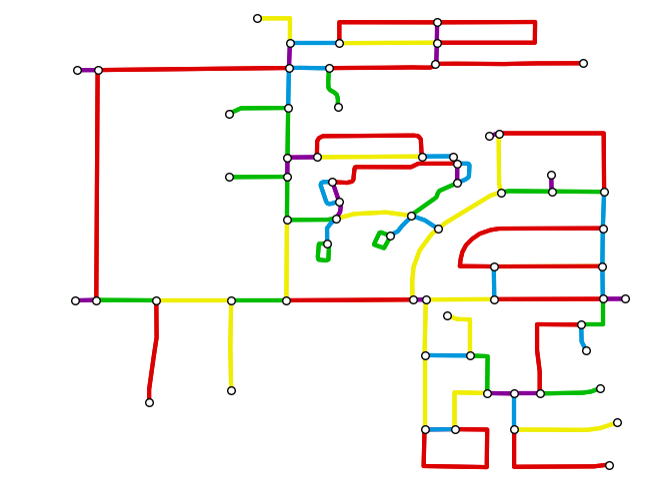
\includegraphics[width=0.4\textwidth]{figures/road-network.png} &
				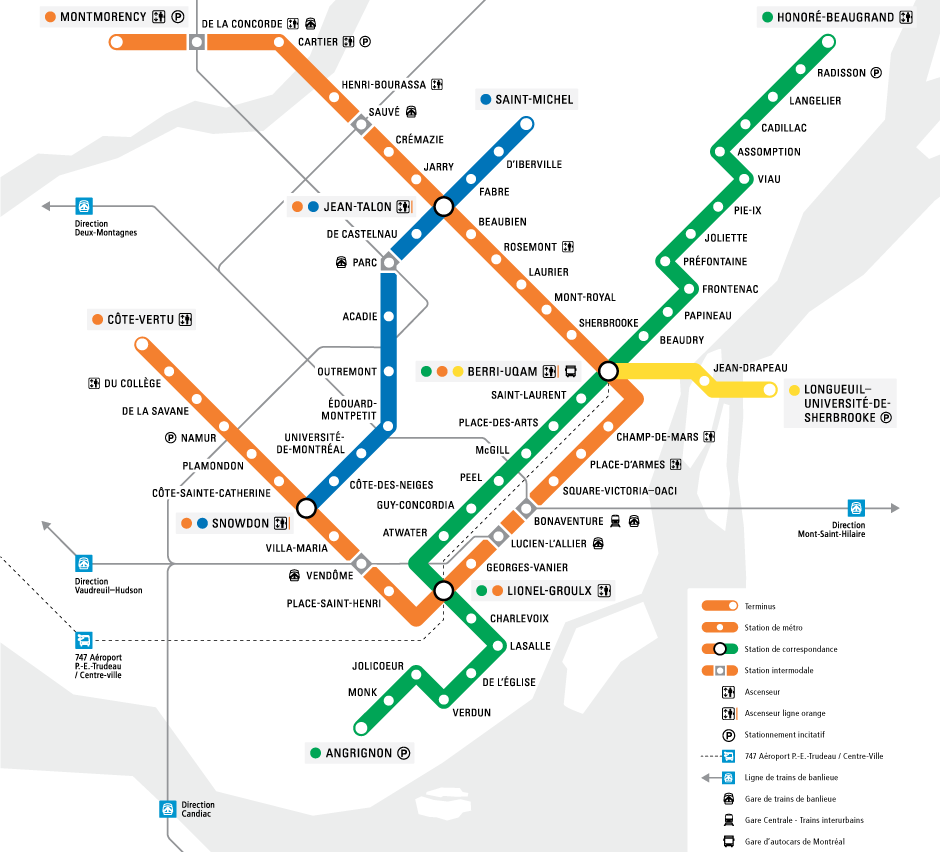
\includegraphics[width=0.4\textwidth]{figures/mtl-metro-cut.png} \\
			\end{tabular}
		\end{center}
		\caption{Example of a typical urban road-based network (left) and a subway route-based network (right).}
		\caption*{\small Sources: \cite{boeing2017osmnx} (left), \url{http://www.stm.info/fr/infos/reseaux/metro} (right)}
		\label{fig:networks}
	\end{figure*}
	
	Massive data collection techniques exist for both of these network contexts, as will be later seen in Section~\ref{sec:dm}, leading to the problem of efficiently handling this vast information. Apart from the usual well-known \textit{Big Data} solutions, there is an ongoing research on the application of data structures for some of these goals. In particular, it is possible to apply many of the techniques from the field of \textit{Compact Data Structures} to build autoindexed representations that support efficient query patterns tailored for specific information needs, while offering some sort of compression with respect of a more traditional representation.
	
	A usable solution would also require a user interface that enables the exploitation of this information by researchers, transportation companies, city administrations and any other kind of end users. This interface must, at the very least, allow visualizing the network elements on a map, also granting the ability to make queries over these elements in an intuitive and responsive way, while respecting the usual quality principles of any user-oriented software of this kind.
	
	\section{Contributions}
	As the two contexts from Section~\ref{sec:pd}~lead to different ways of structuring and querying the information, it is natural to expect at least two different representations, one for each context. For this reason, in this work we have applied some of compact data structures to design novel representations that are able to handle massive collections of data related to user transportation habits. Our proposed representation cover both contexts, as well as offer a fair trade-off for different query needs, while at the same time ensuring that our proposals can be implemented in a real world scenario, for which we evaluate the performance of our representations with realistic query cases over real datasets\footnote{When needed, the real data was augmented or mixed with synthetic information}.
	
	Furthermore, as a proof of the practicability of our approach, we have developed a user interface that is based on our representations, and allows a user to perform queries through a \gls{gis} web interface. Unlike traditional \gls{gis} interfaces, ours is focused on offering convenient methods to query past user trajectories by network elements instead of purely spatial relationships, and achieves far superior performance when compared to systems backed by traditional database systems.
	
	In conclusion, we present an end-to-end platform around representations based on compact data structures to process, store, query and visualize mined public transportation usage data. To our knowledge, this is the first work to accomplish building such integrated platform, although other works exist that contemplate the use of compact data structures for trajectories or moving objects (see Section~\ref{sec:ti}).
	
	\section{Outline}
	This work is structured as follows...
	
\chapter{Related works}
	\section{Data mining}
	\label{sec:dm}
	Currently there are several known techniques that would allow to collect data regarding users' trips over a public transportation network. Numerous works exist where those trajectories are mined from the transactions of smart cards \cite{bhaskar2015passenger,wang2014aggregated}. This can be complemented with information derived from GPS devices, as shown in \cite{ma2014development}. Alternatively, reliable trajectories may be extracted relying on positioning obtained from cellular networks, as proven by \cite{liu2017exploring}.
	
	In order to make significant conclusions about the travel patterns, it is essential to be able to collect a large enough collection of trips to be representative enough of the overall usage within a time span. For this problem, crowd-sourcing can be a viable approach to record the trajectories of public transportation users, as done in \cite{zimmerman2011field}, where the users were rewarded with real information on the bus location, estimation of arrival time and fullness in exchange of recording the GPS trace on their own bus trips.

    Because smart card methods usually provide only information about boarding stops, there are works that study the challenge of inferring alighting stops from passengers \cite{wang2011review}. In addition, the authors of \cite{tao2014exploring} have specifically tackled the challenge of reconstructing full trajectories, accounting for trip-chaining, by using data obtained from smart cards. Furthermore, in \cite{alsger2016validating} it is also proven that not only the alighting stops, but also the (last) destination stop of a trip can be estimated from boarding data gathered by a smart card, within a reasonable accuracy.
    
    This summarized review proves that, although we were not able to access real data from a public transportation company for this work, such curated information about users' trips can indeed be obtained and used for our proposed representations.
	
	\section{Models of trajectory and types of queries}
    There is a large amount of work on designing data models for moving objects~\cite{DBLP:conf/ssdbm/WolfsonXCJ98,DBLP:conf/icde/SistlaWCD97,DBLP:journals/tods/GutingBEJLSV00,DBLP:conf/chorochronos/GutingBEJLNSV03,DBLP:journals/geoinformatica/Spaccapietra01,DBLP:conf/sigmod/ForlizziGNS00,DBLP:journals/geoinformatica/ErwigGSV99,DBLP:books/mk/GutingS2005}. Basically, a moving object data model represents the continuous change of the location of an object over time, this way defining a trajectory.
    
    Moving object can be seen as a big data problem, where solutions may typically differ in the representation of location, contextual or environmental information where the movement takes place, the time dimension, which can be continuous or discrete, and the level of abstraction or granularity on which the trajectories are described~\cite{DBLP:journals/sigspatial/DamianiIGV15}. A common classification of trajectories distinguishes free from network-based trajectories.  \textit{Free trajectories} or Euclidean trajectories are a sequence of GPS points represented by an ad-hoc data type of moving points~\cite{DBLP:conf/ssdbm/WolfsonXCJ98,DBLP:conf/icde/SistlaWCD97,DBLP:journals/tods/GutingBEJLSV00}. \textit{Network constrained} trajectories are a temporal ordered sequence of locations on networks. This trajectory model includes a data type for representing  networks and  for representing the relative location of static and moving  points on the network~\cite{DBLP:journals/vldb/GutingAD06}. When we want to represent trajectories over a road-based network, it is often useful to deal with \textit{network-matched trajectories}, as this will allow to represent large collections trajectories more efficiently. The process of obtaining these network-matched trajectories from GPS points is called \textit{map-matching} \cite{brakatsoulas2005map}. This process can also be done online, as recently shown in~\cite{DBLP:journals/tits/Ding0GL15}, where all the processing is done in the server, eliminating the need of any map or network representation at the moving object side.
    
    The definition of trajectories at an abstract level must be materialized in an internal representation with access methods for query processing. An early and broad classification of spatial-temporal queries for \textit{historical positions} of moving objects \cite{DBLP:conf/vldb/PfoserJT00} identifies coordinate- and trajectory-based queries. Coordinate-based queries include the well-known  {\it time-slice}, {\it time-interval} and \textit{nearest-neighbor queries}. Examples are \textit{find objects or trajectories in a region at a  particular time instant or during some time interval}. Another important example of coordinate-based queries is \textit{find the k-closest objects with respect to a given point at a given time instant}. Trajectory-based queries  involve topology of trajectories (e.g., overlap and disjoint) and information (e.g., speed, area, and heading) that can be derived from the combination of time and space. An example of such queries would be  \textit{find objects or trajectories that satisfy a spatial predicate (eg., leave or enter a region)  at a particular time instant or time interval}. There also exist combined queries addressing information of particular objects: \textit{Where was object X at a particular time instant or time interval}. In all previous queries, the results are individual trajectories that satisfy the query constraints.
    
    %When dealing with large datasets of trajectories, and due to privacy issues, the individual trajectory cannot be revealed, then anonymized and aggregated trajectories are of concern.  
    In many applications, aggregated trajectories must be analyzed in the collection, as an individual trajectory does not represent any useful information.
    In this context, we can  further distinguish range- from trajectory-based queries. Range queries impose constraints in terms of a spatial location  and temporal interval.  Examples of these queries are  to retrieve the number of distinct trajectories  that intersect a spatial region or spatial location (stop) at a given time instant or time interval, retrieve the number of distinct trajectories that start at a particular location (stop) or in a region and/or end in another particular location of region, retrieve the number of trajectories that follow a path, 
     and retrieve the  top-k locations (stops) or regions  with the larger number of  trajectories that  intersect  at a given time instant or time interval. Trajectory-based queries require not only to use the spatio-temporal points of trajectories  but also the sequence of these points. Examples of such queries are  to find the number of trajectories that are heading (not necessarily ending at) to a spatial location during a time interval, find the destination of trajectories that are passing through a region during a time interval, find the number of starting locations of  trajectories that go or pass through a region during a time interval.
	
	\section{Trajectory indexing}
	\label{sec:ti}
	Literature on spatial trajectory indexing can be categorized by the nature of the trajectories: they can be either constrained to a network or in free space (often called moving objects). While there are well-known queries for indexes that work on moving objects in free space \cite{DBLP:conf/vldb/PfoserJT00}, the network constrained trajectory indexes cover more diverse querying needs, as different networks involve different kinds of challenges (as in vehicular road network vs public transportation network), and also because the intended application may vary (analyzing trip-chaining patterns vs number of passengers within a time window). A comprehensive review on indexing methods can be found in \cite[Chapter 4]{DBLP:books/sp/PelekisT14}, to which we shall expand in the rest of this section to mention the most notable indexes and some new developments.
	
	\subsection{Free trajectory indexing}
	Several adaptations of the {\em R-Tree} \cite{DBLP:conf/sigmod/Guttman84} are widely used for the indexing of moving objects. The most common approach is to integrate the temporal dimension in the R-Tree itself, as found in the {\em STR-Tree} and the {\em TB-Tree} from \cite{DBLP:conf/vldb/PfoserJT00}.
    Another common approach is to compliment the R-Tree with another similar structure, as has been done for the {\em MV3R-tree}~\cite{DBLP:conf/vldb/PapadiasT01},
    where an Historical {\em R-Tree}~\cite{nascimento1998towards} to partition on the temporal dimension.
    
    Generally, even for very large collections of trajectories, the spatial dimensions are more bounded than the temporal dimension, which can grow indefinitely. For this reason, even for free trajectories, temporal dimension is generally more selective than spatial dimensions. This observation was heavily exploited in the subsequent works, such as {\em SETI} from \cite{chakka2003indexing}, where the space is partitioned statically, while trajectories are indexed by their temporal dimension using a one dimensional R-Tree, allowing it to grow dynamically.
    
    Recently a framework based on Apache Spark was developed called {\em UlTraMan}~ \cite{ding2018ultraman}, that supports different kinds of partitioning schemes for large collections of trajectories to answer range, kNN or aggregation queries, allowing to repartition the dataset to maximize the query time efficiency for a given query type. Although UlTraMan has been tested over network constrained trajectories, it does not appear to be exploiting network information in any way, hence its inclusion in this category.
    
    In the field of compact data structures, an index called {\em GraCT}~\cite{brisaboa2019gract} has been developed, based snapshots at regular time intervals using {\em k$^2$-Trees}~\cite{brisaboa2009k} and movement logs for individual trajectories to which grammar compression is applied with {\em RePair}~\cite{larsson2000off}. Because of this, GraCT is a self-indexed compact representation that supports spatio-temporal range and nearest-neighbor queries, as well as allowing for direct access to the trajectory information.
	
	\subsection{Network constrained trajectory indexing}
	There are also numerous approaches that use R-Tree based indexes for trajectories that are constrained to an underlying network, aiming to decrease the redundancy in the representation by separating the representation into levels. Examples of such indexes include the {\em FNR-Tree}~\cite{DBLP:conf/ssd/Frentzos03}, where the network elements are indexed with a 2D R-Tree and 1D R-Trees to index time intervals of moving objects along the edges of the network. Some of the limitations of the FNR-Tree are addressed in \cite{DBLP:journals/geoinformatica/AlmeidaG05}, where the authors propose the {\em MON-Tree}, where the moving objects are indexes in two dimensional R-Trees (the dimensions being edge position vs time). More recent alternatives, such as the {\em TMN-Tree}~\cite{chang2010tmn}, integrate {\em B$^+$-Trees}, which have proven to be more space and time efficient for indexing the temporal dimension. Alternatively, in \cite{rivera2018faster} a compact representation of time intervals is proposed using two bitvectors, that can be combined with these R-Tree based indexes to increase the efficiency for temporal filtering. Refer to \cite{john2017performance} for a quick comparison of these R-Tree based indexes.

    As a competitive alternative to these R-Tree based indexes, {\em PARINET}~\cite{DBLP:journals/vldb/PopaZOBV11}, builds spatial partitions from the trajectories based on their distribution and network topology, and uses a B$^+$-Tree to index the trajectories in each partition by time intervals. Although candidate trajectories must be filtered in memory during queries, PARINET is highly efficient in practice as its partitioning strategy minimizes the number of disk accesses needed.
    %The same ideas were used in {\em TRIFL}~\cite{that2015trifl}, where the cost model is adapted for flash storage.
    
    Another relevant representation is described in \cite{DBLP:conf/gis/KroghPTT14}. Their proposed index, {\em NETTRA}, was designed to efficiently solve a specific kind of query called {\em Strict Path Queries (SPQ)}, built on a traditional RDBMS with $B^+$-Tree indexes. Another distinctive feature of NETTRA is its treatment of network constrained trajectories as textual information, which allows to apply string matching techniques such as fingerprinting functions to determine what trajectories have similar paths on their traversed edges. This close equivalence between trajectories and strings has been further exploited by Geodabs~\cite{chapuis2018geodabs}, where both the spatial distribution and sequence information are taken into account for finding trajectories by similarity with fingerprinting. These text-based approaches are sometimes tangled with works on the topic of semantic trajectories such as \cite{al2017semantictraj}.
    
    %For vehicles we also have this \cite{cai2018vector} and \cite{lovell2018lossless}.
    
    A recent compact data structure named {\em CiNCT} has been proposed in \cite{koide2018cinct}, where trajectories are encoded into a string, that is used to build an FM-index \cite{DBLP:conf/focs/FerraginaM00} with a Huffman-shaped Wavelet Tree \cite{ferragina2009compressed}. To further save space, the string is constructed with relative movement labels instead of absolute edges, with an auxiliary structure that represents a network graph built from the input trajectories themselves. While this structure excels at pattern-matching and path extraction in vehicular networks (such as the streets of a city), it cannot be applied to our problems in public transportation networks.
	
\chapter{Previous concepts}
	I am going to develop this more when I have more content on my proposals.
	
	\section{Summed Area Tables}
	The Summed Area Tables were first introduced in computer graphics \cite{crow1984summed} to speed up the mipmapping process.
	
	\section{Entropy coding}
	Introduce Huffman, more importantly, Hu-Tucker, which is like Huffman but preserving lexical order.
	
	\section{Bitvectors}
	Rank and select.
	
	\section{Wavelet Tree and Wavelet Matrix}
	\label{sec:wt}
	\gls{wm} will be less confusing than in my previous paper...
	
	\subsection{Hu-Tucker Wavelet Tree}
	Another way of compressing a $\wt$ is to use a prefix-free variable-length encoding for the symbols. 
For example,  Huffman~\cite{huffman1952method} code can be used to build a
Huffman-Shaped $\wt$~\cite{ferragina2009compressed}, where the tree is not balanced
anymore. The size reduces to $n(H_0(S)+1)+ o(n(H_0(S)+1)) +  O(\sigma \log n)$,\footnote{$O(\sigma \log n)$ term 
includes both the tree pointers and the size of the Huffman model.}   and average time becomes
$O(H_0(S))$ for $rank$, $access$, and $select$  (worst-case time is still $O(\log\sigma)$ 
\cite{Barbay:2013:CPA:2562345.2562626}). By using compressed
bitvectors \cite{{CNO15}} space can be reduced even further to $nH_0(S) +o(n(H_0(S)+1)) +  O(\sigma \log n)$.
Unfortunately, the Huffman codes given to
adjacent symbols are no longer contiguous, and it is not possible to give a $O(\log\sigma)$ bound for
$count(i,j,\alpha,\beta)$ anymore, even if the code is canonical. Hu-Tucker codes~\cite{hu1971optimal}
can be used instead.\footnote{Hu-Tucker ~\cite{hu1971optimal}
	 is an optimal prefix code that preserves the order of the input vocabulary.
	This means that the lexicographic order of the output variable-length binary codes is the same as the order of the input symbols.}
Compression degrades slightly with respect to using Huffman coding,\footnote{Being $L_h$ and $L_{ht}$ the average codeword 
	length of Huffman coding and Hu-Tucker codes respectively, it holds: $H_0 \leq L_h \leq H_0+1$ and $H_0 \leq L_{ht} \leq H_0+2$
	(see \cite{Cover:2006:EIT:1146355} (pages 122-123), or \cite{HORIBE1977148, GilbertandMore1959}).} but the
codes for adjacent symbols are lexicographically contiguous. This permits to solve $count$ efficiently. 
%The size of a Hu-Tucker-shaped $\wt$ ($\wtht$) can be bounded to $n(H_0(S)+2) + o(n(H_0(S)+2)) +  O(\sigma \log n)$ and can be reduced
%to  $n(H_0(S)+1) + o(n(H_0(S)+2)) +  O(\sigma \log n)$ using compressed bitvectors as well.
%\ART{Por que en negritas?}
The size of a {Hu-Tucker-shaped $\wt$} ($\wtht$)  can be bounded to $n(H_0(S)+2) + o(n(H_0(S)+1)) +  O(\sigma \log n)$ and can be reduced
to  $nH_0(S) + o(n(H_0(S)+1)) +  O(\sigma \log n)$ by using compressed bitvectors as well.
	
	\section{Compressed Suffix Array}
	Explaining ST and SA along the way.
	
	\section{GIS interfaces}
	Because I have a web interface with leaflet after all.
	
	
\part{Compact representations}
	\chapter{Representations for public transportation over road-based networks}
	As explained in Section~\ref{sec:pd}, there there are taxis and then there are buses. Their nature is different because of networks, so they must be treated differently. Here we are going to speak about a repr that works better for taxis.
	
	Old ass CTR \cite{brisaboa2018compact} with a WM or WT for times, and we tried different approaches to compress those times. It is not very useful for buses and metro because of the crazy redundancy.
	
	\section{Description}
	Given a transportation network, whether it is formed by road-based or route-based, we work with a representation of the network that is based on a directed graph. For a road-based network, a \textbf{node} represents a road segment delimited by intersections, where two nodes are connected by an edge if it is possible (i.e. legally allowed). This allows to accurately describe a trajectory by sequentially listing the road segments that were traversed, while minimizing the redundancy.
	
	In the other hand, for route-based networks we define the nodes as stops or stations, making two of them connected if there exists a line or route that stops at each, consecutively. We can represent user trajectories following the same strategy as for road-based networks, although that will lead us to redundant representations in most cases. On subway and bus networks it is common to find stops that belong to only one route, and therefore must be either the end of a trajectory or be followed by the only possible next node. Furthermore, a more minimalist representation of a trajectory with the starting, ending and route switching nodes alone would be sufficient to reconstruct the original trajectory. Such representation will be contemplated later in Chapter~\ref{sec:newctr}, while on \gls{ctr} we maintain a common representation strategy for both kinds of networks. Because listing every node traversed introduces redundancy on route-based networks, we state that \gls{ctr} is more adequate for road-based networks.
	
	[speak about queries of interest for road-based]
	
	[trip description with $s$ and $t$]
	
    To support these queries, we need to represent the spatial and temporal components of our collection of user trips $\mathcal{T}$, where each trip is formed by every node traversed. We use a \gls{csa} to represent the spatial component of our dataset of trips within \gls{ctr}. However, we must perform some preprocessing on $\mathcal{T}$ before building a \gls{csa} on it. Initially, we sort the trips by their first node ($s_1$), then by the last node ($s_{l_i}$), then by the starting time ($t_1$), and finally, by its second node ($s_2$), third node ($s_3$), and successive nodes. Note that the start time ($t_1$) of the trip does not belong to the spatial component, but it is nevertheless used for the sorting\footnote{This initial sorting of the trips will allow us to answer some useful queries very efficiently  (i.e., count trips starting at node $X$ and ending at node $Y$).}.
	
	\begin{figure}[h!]
      \begin{center}
      {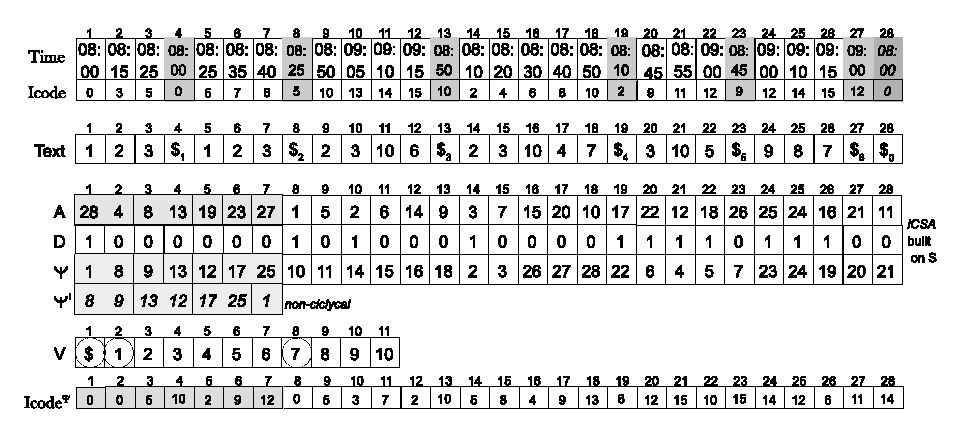
\includegraphics[width=1.00\textwidth]{figures/csttr.eps}}
      \end{center}
      \caption{Structures involved in the creation of a \acrshort{ctr}}
      \label{fig:tcsa}
    \end{figure}
	
	\section{Algorithms}
	We have X to Y and even Top K queries that are not that hard to describe.
	
	\subsection{Time intervals representations}
	Bla bla speak about two alternatives here.
	
	\begin{figure}[htb]
    	\begin{center}
    		{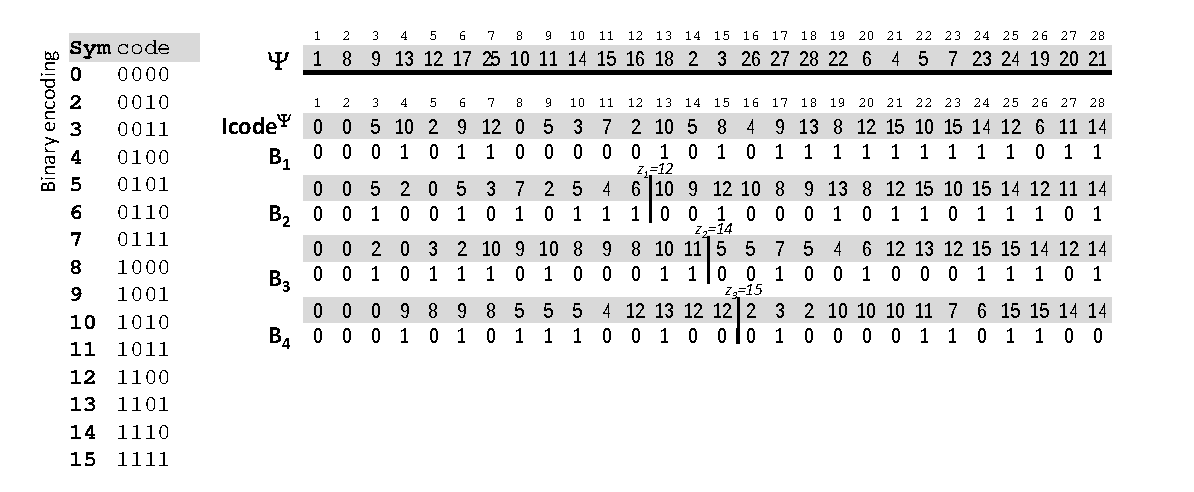
\includegraphics[width=1.0\textwidth]{figures/wma.eps}}
    		{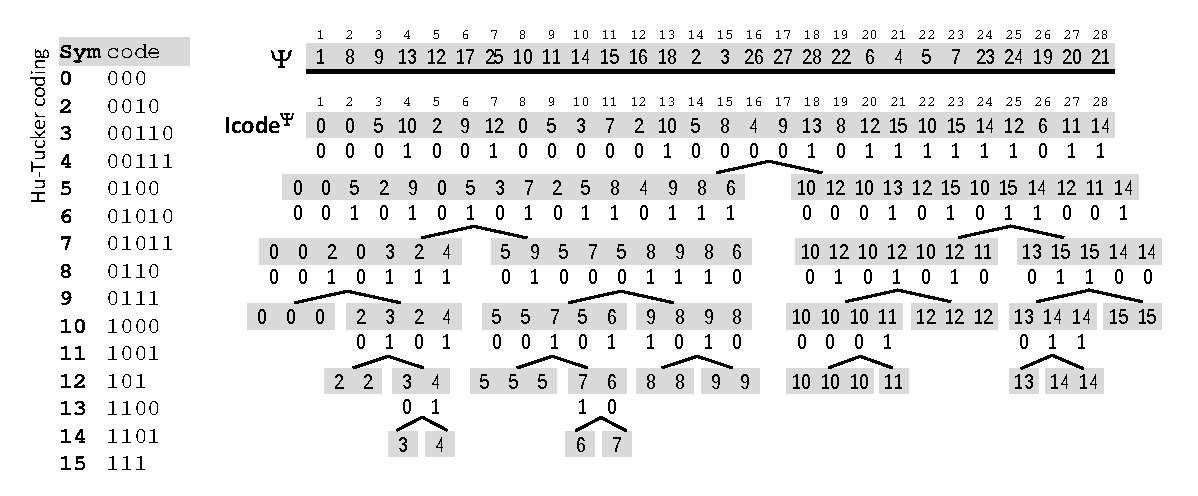
\includegraphics[width=1.0\textwidth]{figures/wta.eps}}
    	\end{center}
    	\caption{Balanced \acrlong{wm} (top) and \acrlong{htwt} (bottom)}
    	%for the times within $Icode^{\Psi}$ in Figure~\ref{fig:tcsa}.}
    	\label{fig:wtwm}
    \end{figure}

	
	Just as proven in Section~\ref{sec:wt} with \gls{wt}, both \gls{htwt} and \gls{wm} implement the $range_{a,b}(S,i,j)$ operation in $O(\log\sigma)$ time on average. This is easy to prove for \gls{htwt} as each node will contain entries from a lexicographically contiguous subrange from the alphabet $\Sigma$, making the same properties seen for \gls{wt} hold. The main difference is that Hu-Tucker codes will reshape the tree, making the leaves containing the least frequent symbols deeper than the leaves with the more frequent symbols, which may theoretically produce a tree of height $\sigma-1$\footnote{Imagine a vocabulary $\Sigma=\{s_1..s_\sigma\}$, where the probability of appearance of the symbol $s_i$ in the text $S$ turned out to be $2^{-i}$.}, which will obviously affect the worst-case performance, in exchange of a very large compression ratio.
	
	The complexity may initially seem harder to analyze for \gls{wm}, as its ``nodes'' are delimited implicitly: the symbols with a code starting in 0 will find their second bit in an implicit node delimited by the subrange $B_2[1..z]$ (for some $1 \leq z < n$), while the symbols with a code starting in 1 will correspond to $B_2[z+1..n]$. Generalizing this idea, we can assert that symbols with the same \textit{context} of $\alpha$ starting bits in their codes will find their next $\alpha+1$ bit in some subrange $B_{\alpha+1}[i..j]$ with $1 \leq i \leq j \leq n$. Therefore, the same properties from \gls{wt} can be exploited for a $range_{a,b}(S,i,j)$ operation in \gls{wm} as well, allowing us to solve it in $O(\log\sigma)$ worst-case time.
	
    While it is possible to build \gls{wm} using canonical Huffman codes, it is unfortunately impossible guarantee the $O(\log\sigma)$ bound on $range_{a,b}(S,i,j)$ on such \gls{wm}, as the symbols lose their original lexicographic proximity, meaning that symbols which would appear on the same node of \gls{wt} due to the common most significant bits in their original codes, would get different Huffman codes based on their frequency of appearance in the text, ending up in separate nodes. On the other hand, to our best knowledge, there is no practical way of building \gls{wm} with Hu-Tucker codes.
	
	\section{Experiments}
	We may have not compared it to anything but we sure do have tons of results!
	
	\chapter{Representations for public transportation over route-based networks}
	\label{sec:newctr}
	This is about a representation that was designed for buses.
	
	Here we speak about TTCTR and XCTR, where we have a network description and index journeys instead of explicit times.
	
	\section{Description}
	A network representation, then CSA for stops. In TTCTR we encode lines in these stops, while in XCTR we make the twist from before (I think) and then separate lines into a WM. Whatever the case, we then have an aligned WM of journeys. Oh and T-Matrices as a DW-like structure.
	
	\section{Algorithms}
	A bit complex for both TTCTR and XCTR. Maybe copy the complexity table from the paper that explains why TTCTR sucks for some queries and we needed to develop XCTR.
	
	\section{Experiments}
	Here we compare one to the other. Maybe include query times for postgresql, maybe later.
	
\part{GIS interface}
	\chapter{GIS interface for public transportation over networks}
	This is an interface that can handle both cases and structures (in theory).
	
	The tool we have developed that can interact with the previously described structures. We retell what we explained about \gls{gis} in previous concepts, and explain that this is different because it is built around our representations.
	
	\section{Architecture}
	From a functional perspective and then a technological one.
	
	\section{API}
	A nice and easy way to make queries and return data.
	
	\section{User Interface}
	With a lot of screencaps that are going to take like 10 pages! Maybe even an evaluation section (which would require me to make it actually work well!).
	
\chapter{ Conclusions and future works}
	2-3 pages to speak about lessons learned and where is this all going. Speak about field tests with people from Caminos...

% \nocite{*}
% \bibliographystyle{apalike}
\bibliographystyle{alpha}
\addcontentsline{toc}{chapter}{\bibname}
\bibliography{thesis}

\vfill \pagebreak \thispagestyle{empty} \mbox{}
\vfill \pagebreak \mbox{} \thispagestyle{empty}

\end{document}
%###
